\chapter{Constrained Clustering}\label{ch:ConstrainedClustering}

Having introduced the basic concepts of clustering, the aim of this chapter is to define the concepts related to constrained clustering, as well as to give examples of its application and highlight the benefits and problems presented by its use. To this end we take as our main reference the survey presented in \cite{davidson2007survey}.

\section{Motivation for Constrained Clustering}

As we discussed in Chapter \ref{ch:IntroClustering}, unsupervised clustering methods are useful for structuring data referring to a particular area. An example of this can be found in text classification; In \cite{cohn2003semi} a problem proposed by Yahoo! is faced. The problem consist of, given a large number of text documents, grouping them according to a taxonomy in which documents with similar topics are nearby. For this, unsupervised clustering methods are useful, as the information on the problem initially available is limited. However, in \cite{wagstaff2001constrained} is shown that applying unsupervised clustering to certain problems, such as grouping GPS data in such a way that clusters define the lanes of a road, does not produce significant results, as the clusters obtained are far from the elongated shape that would be expected as a result. To tackle the problem, they introduced a new element in clustering, the instance-level constraints, which made it possible to include knowledge about the clusters that would guide the clustering methods to obtain the expected results. It was enough to indicate that the lanes of the road on which the vehicles circulate are four meters wide, and therefore any vehicle that is at a distance of more than 4 meters from another, perpendicular to the direction of displacement, must be located in a different cluster.

We are now in a new scenario: it is possible to incorporate additional information to the clustering process, in addition to that contained in the data set itself, to guide it in the formation of the partition and obtain more precise results. This places constrained clustering in the framework of semi-supervised learning, unlike traditional clustering methods which fall within the area of unsupervised clustering. 

\section{Constraints Definition}

The new type of information that we incorporate to clustering is given in the form of instance-level constraints, that is, to specify if two instances ($x_i$ and $x_j$) from the dataset ($X$) must be in the same cluster or, on the contrary, they must be in separate clusters.

Constraints that indicate that two instances must be placed in the same cluster are called \acf{ML}, and are noted with $C_=(x_i,x_j)$. Similarly, constraints that specify that two instances must not be placed in the same cluster are called \acf{CL}, and are noted with $C_{\neq}(x_i,x_j)$ \cite{wagstaff2000clustering}.

Although they may seem simple, constraints defined as above have some very interesting properties. Must-link constraints are an example of an equivalence relationship, and therefore are symmetrical, reflexive and transitive, formalizing:

\begin{observation}
	\textbf{Must-link constraints are transitive.} Let $CC_i$ and $CC_j$ be connected components (completely connected subgraphs by \acs{ML} constraints), and let $x_i$ and $x_j$ be the instances in $CC_i$ and $CC_j$ respectively. Then $C_=(x,y): x \in CC_i, y \in CC_j \rightarrow C_=(a,b) \forall a,b: a\in CC_i, b \in CC_j$. \cite{davidson2007survey}
\end{observation}

\begin{observation}
	\textbf{Cannot-link constraints can be entailed.} Let $CC_i$ and $CC_j$ be connected components (completely connected subgraphs by \acs{CL} constraints) and let $x_i$ and $x_j$ be the instances in $CC_i$ and $CC_j$ respectively. Then $C_{\neq}(x,y): x \in CC_i, y \in CC_j \rightarrow _{\neq}(a,b) \forall a,b: a\in CC_i, b \in CC_j$. \cite{davidson2007survey}
\end{observation}

A clear example of constraint use can be found in clustering applications where there are distance measurement limitations, as in the case of GPS data. Thus, if we want that instances forming two clusters to be separated by a distance greater or equal to $\delta$, it is enough to set \acs{ML} constraints between all instances separated by less than $\delta$ units. Similarly, if we want the diameter of the clusters to be at most $\epsilon$, we must set \acs{CL} constraint between instances separated by more than $\epsilon$ units. Figure \ref{fig:DistanceConstraints} shows a graphical representation of these two types of constraints.

\begin{figure}[!h]
	\centering
	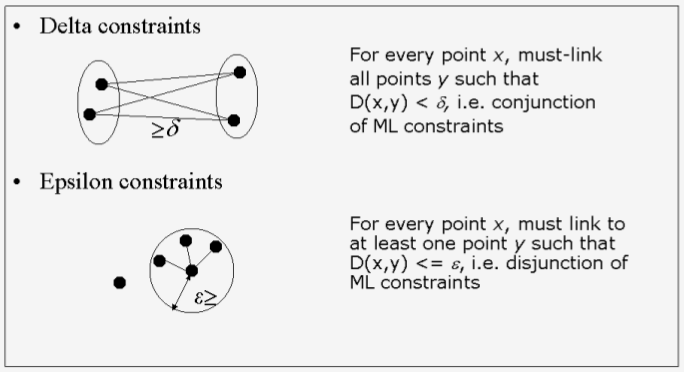
\includegraphics[scale=0.45]{gfx/ConstClust/RestriccionesDeltaEpsilon.png} 
	\caption[\textit{delta} and \textit{epsilon} constraints]{\textit{delta} and \textit{epsilon} constraints \cite{davidson2007survey}.}\label{fig:DistanceConstraints}
\end{figure}


\section{Use of Constraints}

While supervised learning involves knowing the label associated with each instance, \acf{SSL} has only a subset of tagged instances. On the other hand, in many domains the available information refers to relations between instances, and not to the specific class to which they belong. Moreover, in interactive clustering systems, a user who is not expert in the domain of the problem will probably be able to provide information in the form of constraints such as \acf{ML} and \acf{CL}. \cite{cohn2003semi}\cite{davidson2007hierarchical}, rather than providing information on what particular class certain instances belong to.

Typically, constraints are incorporated into clustering problems in two ways. They can be used to alter the instance clusters assignment rule of the method in hand, so that the solution satisfies as many constraints as possible. Alternatively, it is possible to train the distance function used by the method based on the constraints, either before or during the application of the method. In any case, the initialization phase can take the constraints into account, so that instances associated with constraints \acf{ML} will be placed in the same cluster, and those between which there is a constraint \acf{CL} will be placed in different clusters. Based on this distinction, we identify two ways of approaching the problem, those based on constraints (\textit{constraint-based}), and those based on distances (\textit{distance-based}).

\subsection{Constraints-based Methods}

In constraint-based methods, the clustering method itself is modified in such a way that the available information is used to bias the search and obtain an appropriate data partition.

Regarding the degree to which the constraints have to be satisfied, we can make a distinction between the concepts of hard \cite{wagstaff2001constrained}\cite{davidson2005agglomerative} and soft \cite{law2004clustering}\cite{basu2004active}\cite{segal2003discovering}\cite{davidson2005clustering}\cite{law2005model} constraints. Hard constraints must necessarily be satisfied in the output partition of any algorithm that makes use of them, while soft constraints are taken as a strong guide for the algorithm that uses them but can be partially satisfied in the output partition \cite{seret2014new}. For the purposes of this work, we will employ the latter. There are several techniques to obtain a partition based on constraints:

\begin{itemize}
	
	\item  Modify the objective function to include a penalty term for breaking constraints \cite{demiriz1999semi} \cite{davidson2005clustering}.
	
	\item Group instances with additional information obtained from a conditional distribution into an auxiliary space \cite{sinkkonen2000semisupervised}.
	
	\item Enforcing all constraints to be satisfied by modifying the the instance clusters assignment rule \cite{wagstaff2001constrained}.
	
	\item Initialize clusters based on constraints inferred from a set of labeled instances \cite{basu2002semi}.
	
\end{itemize}

Figure \ref{fig:ConstOverDataset} shows a data set together with its associated constraints. Figure \ref{fig:ClusteringSatAllConst} proposes a possible clustering that satisfies all constraints.

\begin{figure}[bth]
	\myfloatalign
	{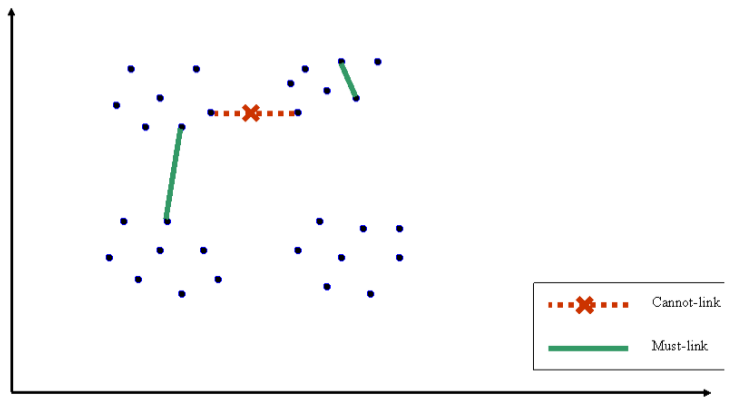
\includegraphics[width=.6\linewidth]{gfx/ConstClust/InputInstancesAndConst1}
	\caption[Constraints on a dataset.]{Constraints on a dataset. \cite{davidson2007survey}} \label{fig:ConstOverDataset}
	}
	{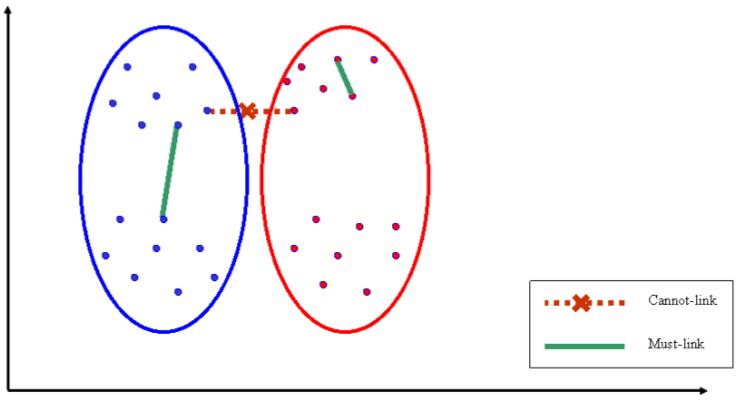
\includegraphics[width=.6\linewidth]{gfx/ConstClust/ClusteringSatAll}
	\caption[Clustering satisfying all constraints.]{Clustering satisfying all constraints. \cite{davidson2007survey}} \label{fig:ClusteringSatAllConst}
	}
\end{figure}

\subsection{Distance-based Methods}

In distance-based approaches, classic clustering methods that use a distance measurement are employed, so that the distance measurement is modified to incorporate the constraints. In this context, satisfying constraints means that instances related to constraints \acf{ML} are placed together in the space, and those related by \acf{CL} are separated.

Figure \ref{fig:MetricLearned} shows a possible clustering based on a metric learned from the constraints specified in Figure \ref{fig:ConstOverDataset2}. It should be noted that in Figure \ref{fig:MetricLearned} the space in which the data is located has been compressed on the vertical axis and widened on the horizontal axis to match the learned distance metric.

\begin{figure}[bth]
	\myfloatalign
	{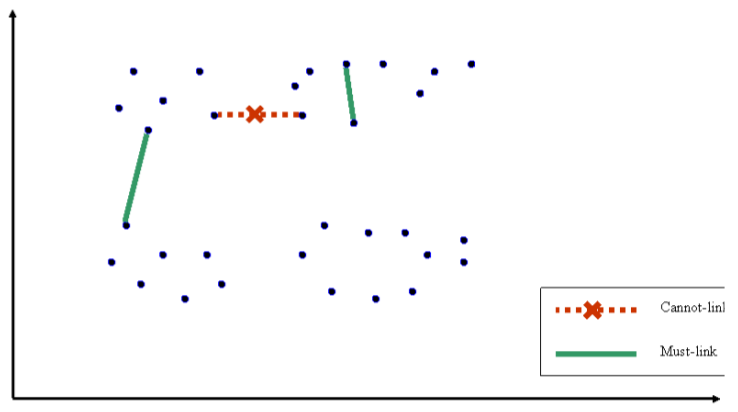
\includegraphics[width=.6\linewidth]{gfx/ConstClust/InputInstancesAndConst2}
	\caption[Constraints on a dataset.]{Constraints on a dataset. \cite{davidson2007survey}} \label{fig:ConstOverDataset2}
	}
	{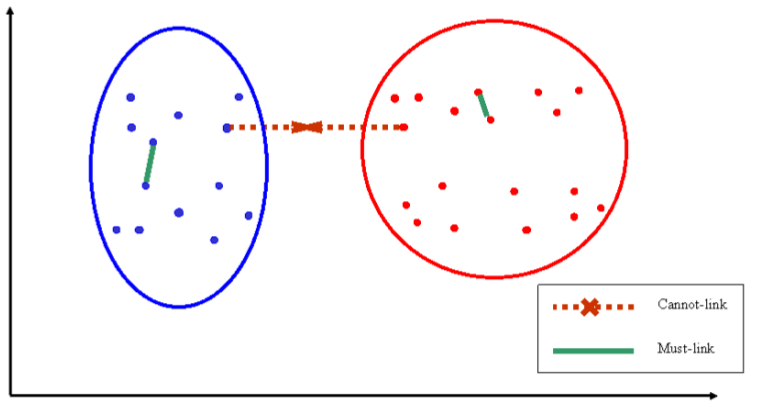
\includegraphics[width=.6\linewidth]{gfx/ConstClust/MetricaAprendida}
	\caption[Clustering based on a metric learned based on constraints.]{Clustering based on a metric learned based on constraints. \cite{davidson2007survey}} \label{fig:MetricLearned}
	}
\end{figure}

\section{Constrained Clustering Applications} \label{sec:CCApplications}

This section shows some application cases in which constrained clustering has turned out to be a more useful tool than unsupervised clustering. For each case we will analyze how the constraints were obtained and how they improve the results in the resulting clustering. 

\subsection{Image Analysis}

Figure \ref{fig:CMUFacesDatabase} shows a sample from the CMU (Carnegie Mellon University) faces dataset, where the task is to group faces based on different criteria. In this case, the goal is to group the faces according to their orientation.

\clearpage

\begin{figure}[bth]
	\myfloatalign
	\subfloat[Profile faces.]
	{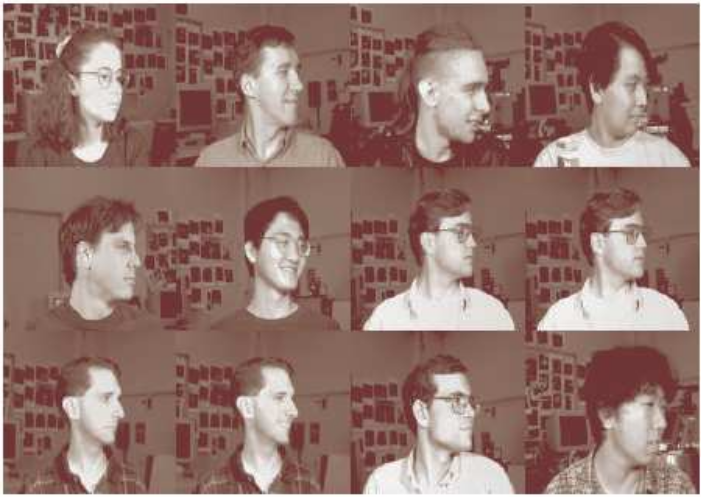
\includegraphics[width=.3\linewidth]{gfx/ConstClust/AnalisisImagenes/Caras1}} \quad
	\subfloat[Front faces.]
	{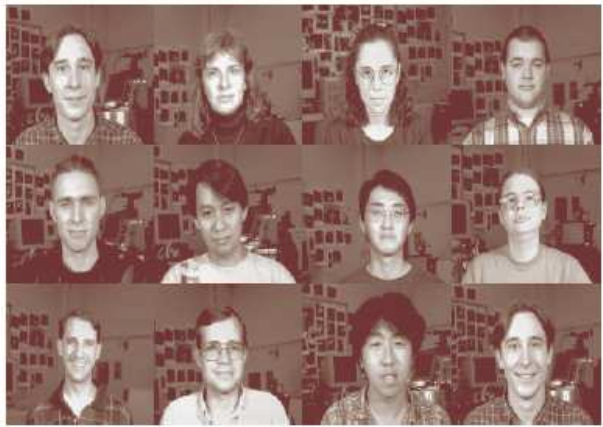
\includegraphics[width=.3\linewidth]{gfx/ConstClust/AnalisisImagenes/Caras3}} \quad
	\subfloat[Faces up.]
	{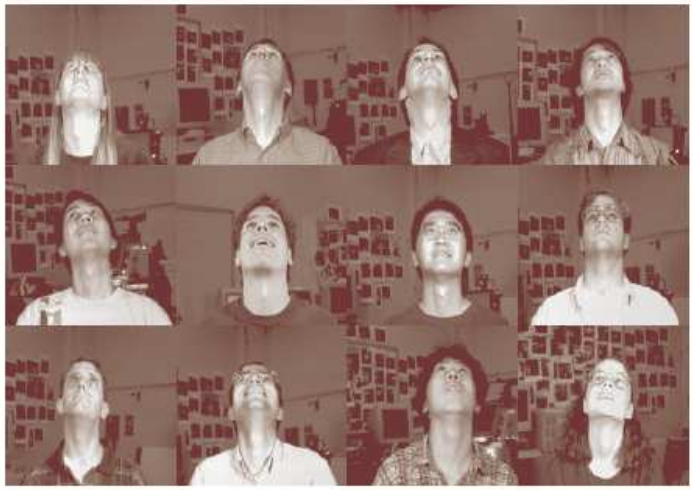
\includegraphics[width=.3\linewidth]{gfx/ConstClust/AnalisisImagenes/Caras2}} \quad
	\caption[CMU database faces.]{CMU database faces. \cite{davidson2007survey}}\label{fig:CMUFacesDatabase}
\end{figure}

The method used to obtain the constraints is one of the most popular in the literature: set the number of clusters of the resulting partition equal to the number of classes in the database, and generate the constraints from a subset of tagged instances; that is, if two instances have different labels, set a \acf{CL} constraint between them, otherwise one of \acf{ML} type. Thus, between the images shown in Figure \ref{fig:FacesDatabaseCL} \acf{CL} constraints are set, since, although they belong to the same person, they do not have the same orientation.

\begin{figure}[bth]
	\myfloatalign
	{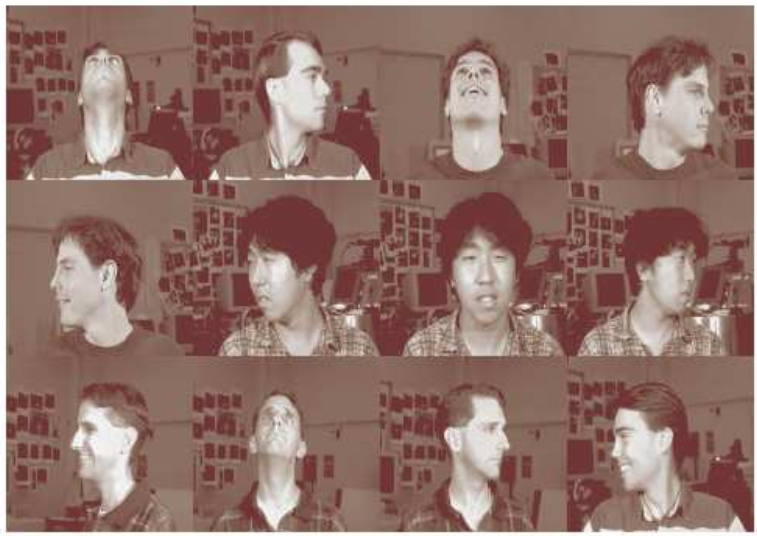
\includegraphics[width=.35\linewidth]{gfx/ConstClust/AnalisisImagenes/CarasDifOr1}} \quad
	{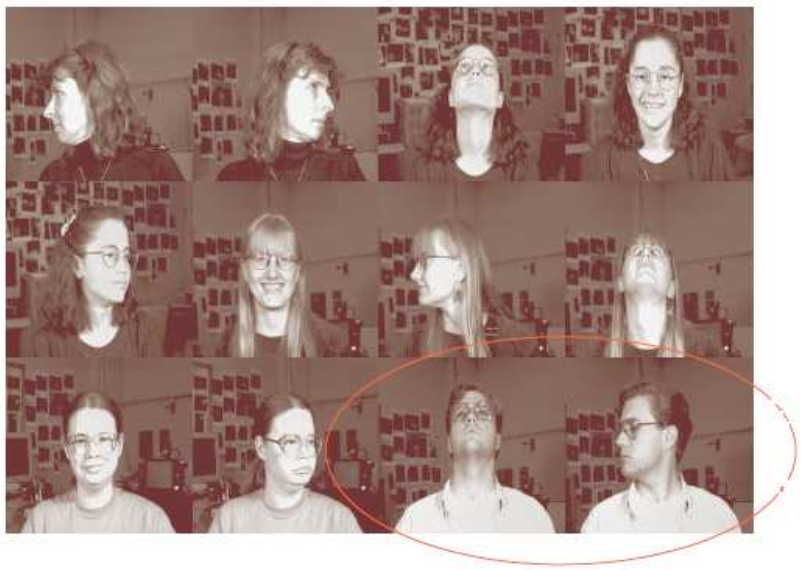
\includegraphics[width=.35\linewidth]{gfx/ConstClust/AnalisisImagenes/CarasDifOr2}}
	\caption[\acs{CL} constraints between faces of the same person.]{\acs{CL} constraints between faces of the same person. \cite{davidson2007survey}}\label{fig:FacesDatabaseCL}
\end{figure}

Figure \ref{fig:AiboRobotClustSys} shows another set of image data on which constrained clustering techniques are applied. In this case, the task is to perform object recognition to incorporate the method into the navigation system of the Aibo robot \cite{davidson2005clustering}. Distance constraints such as $\delta$ and $\epsilon$ are used as described in Figure \ref{fig:DistanceConstraints}. In this way well differentiated clusters are obtained and therefore they are useful for the path-finding techniques performed by the robot during navigation.

\begin{figure}[bth]
	\myfloatalign
	\subfloat[Imagen original]
	{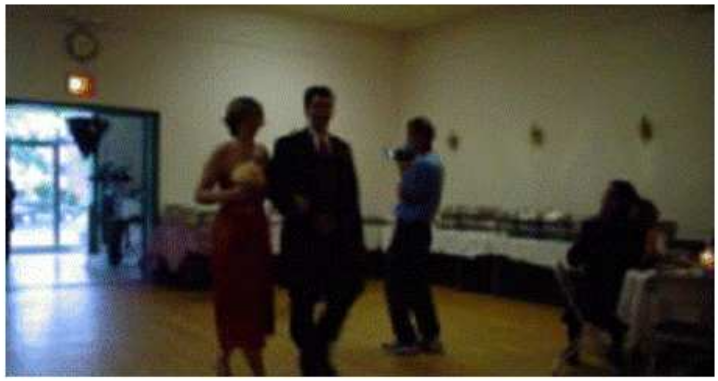
\includegraphics[width=.3\linewidth]{gfx/ConstClust/AnalisisImagenes/Aibo1}} \quad
	\subfloat[Clustering sin restricciones]
	{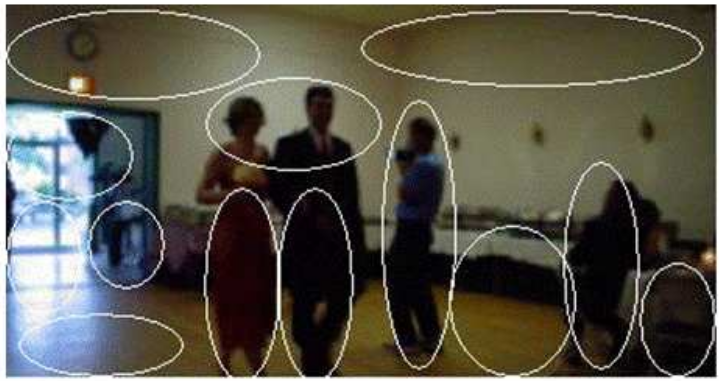
\includegraphics[width=.3\linewidth]{gfx/ConstClust/AnalisisImagenes/Aibo2}} \quad
	\subfloat[Clustering con restricciones]
	{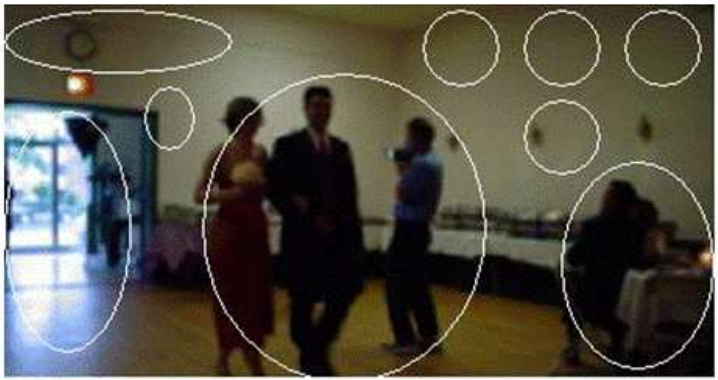
\includegraphics[width=.3\linewidth]{gfx/ConstClust/AnalisisImagenes/Aibo3}} \quad
	\caption[Clustering method used in Aibo Robot navigation system.]{Clustering method used in Aibo Robot navigation system. \cite{davidson2007survey}\cite{davidson2005clustering}}\label{fig:AiboRobotClustSys}
\end{figure}

\subsection{Video Analysis}

Video databases are one example where constraints can be generated directly from the data domain, especially if space-time data information is available \cite{yan2006discriminative}. In time sequenced data it is possible to set \acf{ML} constraints between groups of pixels of frames close in time. This is especially useful when the task is to perform object recognition based on clustering and segmentation. It is also possible to add \acf{CL} constraints to image segment in the same snapshot, as there is a low probability that they are associated with the same object after segmentation is done. In fact, in the video analysis domain problems there are a variety of constraint extraction methods \cite{yan2006discriminative}, Figure \ref{fig:ConstExtractionVideo} shows some examples. 

\begin{figure}[bth]
	\myfloatalign
	\subfloat[]
	{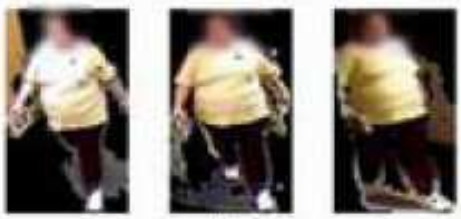
\includegraphics[width=.4\linewidth]{gfx/ConstClust/Videos/VideoA}}
	\quad
	\subfloat[]
	{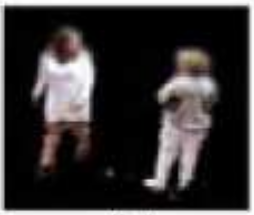
\includegraphics[width=.225\linewidth]{gfx/ConstClust/Videos/VideoB}} \quad
	\subfloat[]
	{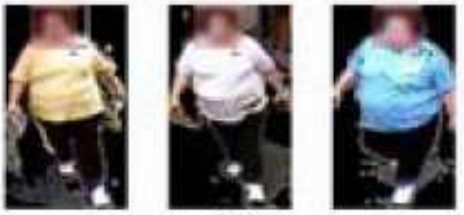
\includegraphics[width=.4\linewidth]{gfx/ConstClust/Videos/VideoC}}
	\quad
	\subfloat[]
	{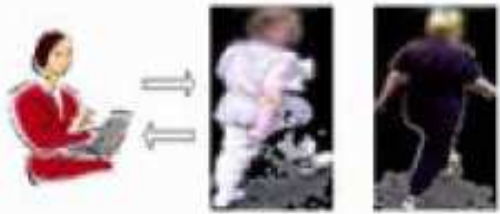
\includegraphics[width=.4\linewidth]{gfx/ConstClust/Videos/VideoD}}
	\caption[Constraints extraction in video data.]{Constraints extraction in video data. \cite{yan2006discriminative} \cite{davidson2007survey}}\label{fig:ConstExtractionVideo}
\end{figure}

In Figure \ref{fig:ConstExtractionVideo}, image (a) corresponds to constraints extracted from tracking a person over a period of time, (b) corresponds to spatial constraints associating two objects located in the same frame, image (c) corresponds to restrictions obtained through facial recognition and (d) to those provided by the user.

With so many constraint extraction methods, one might ask: what happens if too many constraints are imposed? Does this make the problem over-constrained? In Section \ref{sec:ConstraintsProblems} we will address these questions.

\subsection{Biological Data}

In gene clustering based on micro-array data, genes are represented by their expression profile in different experiments and grouped using different methods, in this case constrained clustering methods. Figure \ref{fig:GeneticApp} shows an example: these are \acf{ML} constraints set between genes based on co-occurrence data stored in the protein interaction database, which contains information about which genes (and their associated proteins) are present in the same cell processes \cite{xenarios2001dip}. This information can be used to improve results provided by clustering methods. \cite{segal2003discovering}.

\begin{figure}[!h]
	\centering
	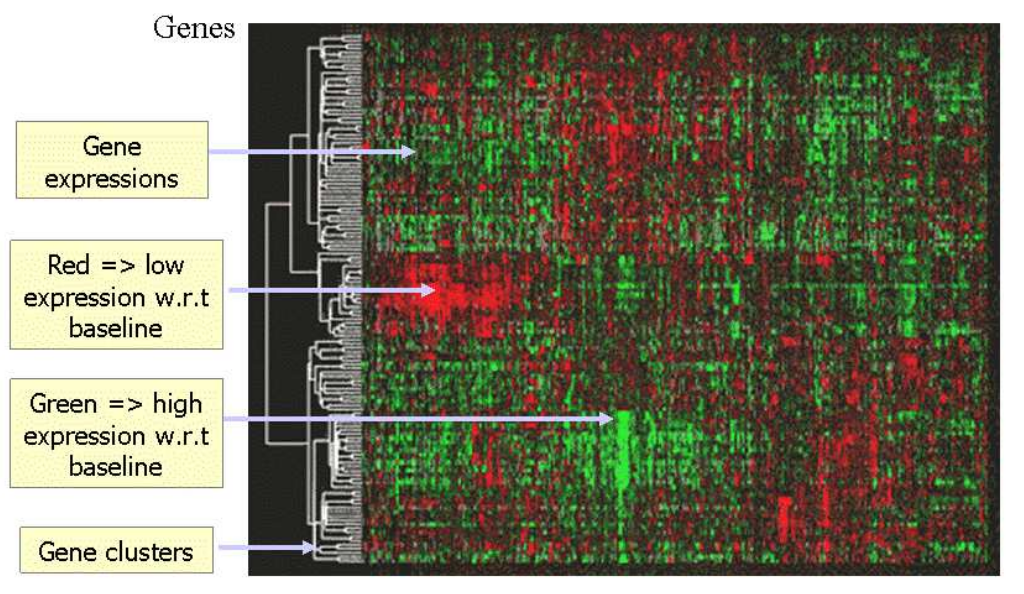
\includegraphics[scale=0.3]{gfx/ConstClust/Genetica/Genes} 
	\caption[Gene clustering based on micro-array data.]{Gene clustering based on micro-array data. \cite{davidson2007survey}}\label{fig:GeneticApp}
\end{figure}

\subsection{Text Analysis}

In content classification tasks, the goal is to automatically split large amounts of documents into groups or clusters. In this case it is possible to extract constraints from multiple auxiliary resources. For example, if two documents are in the same directory, a \acf{ML} constraints could be set between them. This way it is possible to adjust the resulting clustering to suit a particular criterion, such as creating a hierarchy of documents similar to the way they are organized in the input directories structure.

\subsection{Web Data} 

El clustering con restricciones resulta de gran utilidad en el procesamiento de datos de búsqueda en páginas web. Aquí, el objetivo es agrupar, de manera automática, los resultados de una consulta ambigua en el motor de búsqueda en clusters de \acs{URL}s, que se refieran al concepto introducido como consulta en diferentes contextos. En este ámbito es posible extraer las restricciones a partir de búsquedas realizadas anteriormente por los usuarios, de manera que se establece una restricción de tipo \acf{ML} entre \acs{URL}s visitadas en la misma sesión de usuario. Aplicar clustering utilizando estas restricciones puede ayudar a sesgar el resultado de las búsquedas hacia las preferencias del usuario.

\subsection{Aplicaciones en datos de audio}

Constrained clustering is very useful in the processing of search data on web pages. Here, the aim is to automatically group the results of an ambiguous query in the search engine into clusters of \acs{URL}s, which refer to the concept introduced as a query in different contexts. In this area it is possible to extract constraints from searches previously performed by users, so that a \acf{ML} constraint is set between visited \acs{URL}s in the same user session. Clustering using these constraints can help biasing search results towards user preferences.

\subsection{Aplicaciones en datos de GPS} \label{sec:GPSApp}

As mentioned at the beginning of Chapter \ref{ch:ConstrainedClustering}, constrained clustering can be applied to \acs{GPS} data to identify the lane in which each vehicle is running, as shown in Figure \ref{fig:GPSClustData}. Each instance is represented by the position it occupies on the road in two-dimensional Cartesian coordinates $(x,y)$, obtained from \acs{GPS} data. Figure \ref{fig:figure15} graphically shows this representation of the data (note that multiple instances can refer to the same vehicle at different times).

\begin{figure}[!h]
	\centering
	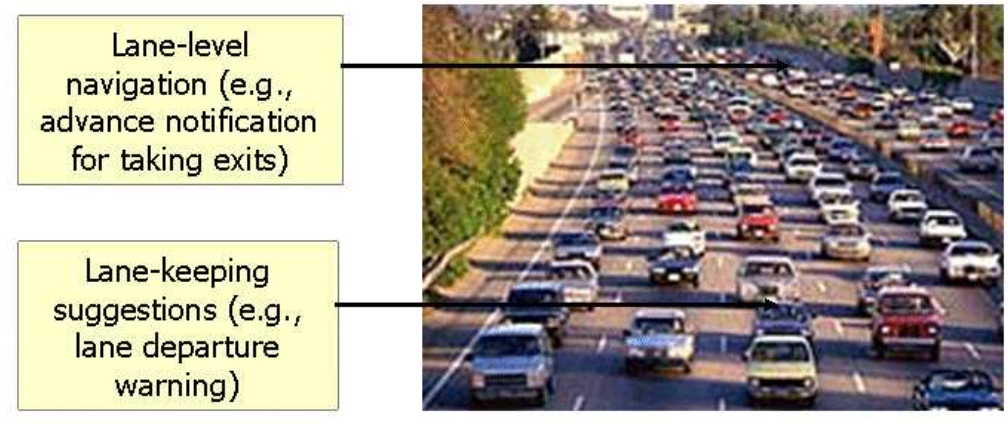
\includegraphics[scale=0.3]{gfx/ConstClust/GPS/Coches} 
	\caption[GPS data use.]{GPS data use. \cite{davidson2007survey} \cite{wagstaff2001constrained}}\label{fig:GPSClustData}
\end{figure}


In this domain, real clusters have an elongated shape on the horizontal axis and are aligned perpendicularly to the motion direction. To get the resulting clusters to have this shape, we can make use of the constraints. We will set a \acf{CL} constraint between those instances more than 4 meters perpendicularly to the motion direction (since the lanes have a maximum width of 4 meters), and \acf{ML} constraints between those instances that present continuity in the motion direction axis, since it is likely that the vehicles they represent are in the same lane. This clustering model has proven to be very useful in real-time navigation \cite{wagstaff2001constrained}, allowing the user to be notified when to change lanes, or when not to leave them.

\begin{figure}[!h]
	\centering
	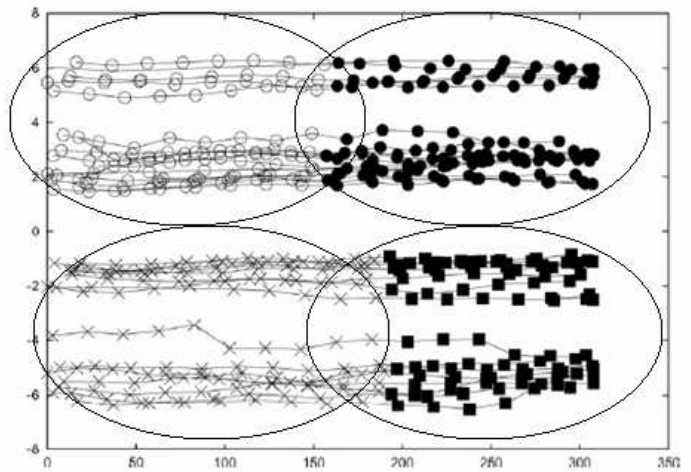
\includegraphics[scale=0.32]{gfx/ConstClust/GPS/Instancias} 
	\caption[Resulting Clustering from GPS data with no constraints.]{Resulting Clustering from GPS data with no constraints. \cite{davidson2007survey} \cite{wagstaff2001constrained}}\label{fig:figure15}
\end{figure}

\subsection{Recent Applications}

The named constrained clustering applications are the most studied in the literature, but it is worth noting that is has been applied to many other fields in recent times. The following is a list of some of those applications: advanced robotics applications \cite{davidson2005clustering, semnani2016constrained}, applied marketing \cite{seret2014new}, obstructive sleep apnea analysis \cite{mai2018evolutionary}, handwritten digits classification \cite{li2015scalable}, Internet traffic classification \cite{wang2014internet}, electoral district designing, \cite{brieden2017constrained}, among others. \textcolor{red}{Poner mas ejemplos de aplicación recientes}

\section{Benefits of Using Constraints}

Two main benefits are found in the use of constraints:

\begin{itemize}
	
	\item Increased accuracy in label predictions by generating constraints based on a subset of labeled instances.
	
	\item Obtaining clusters with adaptable geometry to each problem.
	
\end{itemize}

These two benefits are discussed below:

Given $X = \{x_1 \cdots x_u\}$, a large set of unlabeled instances, and $L = \{(x_{u+1}, y_{u+1}) \cdots (x_{u+l}, y_{u+l})\}$, a small set of labeled instances, it is common to choose two elements from $L$ (with replacement) and set a \acs{ML} constraint between them if they belong to the same class, or a \acs{CL} constraints otherwise. An appropriate method to evaluate the results provided by a clustering method is to measure the level of accuracy of this when predicting dataset $X$ labels. This normally requires specifying the number of desired clusters equal to the number of known classes in $X$ ($k = k^*$). Methods such as the RandIndex \cite{rand1971objective} or its variants, which will be discussed later, are used to measure the degree of agreement between two given partitions (clusterings).

In \cite{wagstaff2000clustering}, where constraints are generated as described above, it is shown that, when an average of the accuracy of the predictions obtained with constrained clustering algorithms is made, varying the latter between experiments, results are obtained up to 20\% better than with classical clustering techniques.

\begin{observation}
	
	\textbf{Using constraints increases accuracy on average.}
	The performance of a method in predicting labels increases when averaged using numerous different constraint sets. \cite{davidson2007survey}
	\label{ob:AccuracyIncrease}
	
\end{observation}

This rule, however, is not true in all cases, as in data sets such as \textit{Tic-Tac-Toe Endgame}, no increase in predictions is achieved regardless of the number of constraints used. A possible explanation for these exceptions is based on the fact that setting $k = k^*$ is not appropriate in these cases.

The other benefit of using constraints is the possibility of obtaining clusters with the desired geometry, such as the example of \acs{GPS} data clustering, analyzed in the Section \ref{sec:GPSApp}.

\section{Problems of Using Constraints} \label{sec:ConstraintsProblems}

Although, as we have seen, the incorporation of constraints to clustering methods brings benefits in some applications, there are two main drawbacks that are discussed below, as well as possible solutions to them.

\subsection{The Feasibility Problem}

Introducing constraints in clustering changes the problem it solves, which becomes: \textit{Find the best partition that satisfies all constraints}. This way, if constraints are not properly specified or if the extraction methods are inadequate, we can find that the constraints contradict each other, which means that there is no partition that satisfies them all. For instance, there is no partition that satisfies the constraints $C_=(x_i,x_j)$ and $C_{\neq}(x_i,x_j)$, regardless of the value of $k$. The same happens for $k = 2$, and the constraints $C_{\neq}(x_i, x_j)$, $C_{\neq}(x_j, x_q)$ and $CL(x_i, x_q)$. Definition \ref{def:FeasibilityProblem} formalizes the feasibility problem for non-hierarchical instance-level constrained clustering:

\begin{definition}
	
	\textbf{Feasibility problem for non-hierarchical instance-level constrained clustering:} Given a dataset $X$, a constraint set $CS$, and the bounds on the number of clusters $k_l \leq k \leq k_u$, does there exist a partition $C$ of $X$ with $k$ clusters such that all constraints in $CS$ are satisfied? \cite{davidson2005clustering} \cite{davidson2007survey}
	
	\label{def:FeasibilityProblem}
	
\end{definition}

 The theoretical complexity of a constrained clustering problem depends on the type of constraints combined in it. Table \ref{tab:CCComplexity} summarizes the expected complexity in each case. 

\begin{table}[!h]
	\centering
	%\setlength{\arrayrulewidth}{1mm}
	\setlength{\tabcolsep}{7pt}
	\renewcommand{\arraystretch}{1.2}
	%\resizebox{\textwidth}{!}{
	\begin{tabular}{ >{\centering\arraybackslash}m{4cm}  >{\centering\arraybackslash}m{4cm} }
		\hline
		\textbf{Constraints} & \textbf{Complexity} \\
		$\delta$ & $\mathbf{P}$ \\
		$\epsilon$ & $\mathbf{P}$ \\
		\acs{ML} and $\delta$ & $\mathbf{P}$ \\
		\acs{ML} and $\epsilon$ & $\mathbf{NP}$-complete \\
		$\epsilon$ and $\delta$ & $\mathbf{P}$ \\
		\acs{CL} and other & $\mathbf{NP}$-complete \\
		\hline
		
	\end{tabular}%}
	\caption[Complexity of the constrained clustering problem depending on the type of constraints.]{Complexity of the constrained clustering problem depending on the type of constraints. \cite{davidson2007survey}}
\label{tab:CCComplexity}
\end{table}

As shown in Table \ref{tab:CCComplexity}, the use of \acf{CL} constraints increases the constrained clustering complexity level to $\mathbf{NP}$-complete and therefore constrained clustering is intractable. Intuitively it can be easily understood that if finding a single partition that satisfies the constraints is a complex problem, finding the best of them is harder.

\begin{observation}
	
	\textbf{Knowing a feasible solution exists does not help us find it.} The consequences of this result on the constrained clustering complexity imply that, even if there is a feasible partition, it will not be easy to find, speaking in terms of algorithmic complexity \cite{davidson2007survey}.
	\label{ob:FeasibleSolution}
	
\end{observation}

In \cite{wagstaff2002intelligent} and \cite{davidson2007hierarchical} is shown that, even in the number of clusters in the output partition is set equal to the number of classes in the dataset ($k = k*$), which guarantees that a feasible solution does exists, simple algorithms like the COP-kmeans \cite{wagstaff2001constrained} may not converge due to the feasibility problem.

\subsection{The Constraint Set Utility Problem} \label{sec:UtilityProblem}

In constrained clustering it is assumed that constraints are a guide for an algorithm to find de desired data partition. So, it is reasonable to think that the more additional information (constraints) we have available, the closer the result we get to the one we are looking for, as Observation \ref{ob:AccuracyIncrease} stated. However, and despite the stipulations of this observation, we find cases in which, even generating the constraints without noise and on the basis of the true labels, there are constraint sets that, far from improving the results, worsen them considerably \cite{davidson2006proceedings}. This seems to disagree with the Observation \ref{ob:AccuracyIncrease}, however, let us remember that it refers to the average case, and not to particular cases.

\begin{observation}
	
	\textbf{Individual constraint sets can have adverse effects}. Some constraint sets generated on the same ground truth labels that evaluate the clusters can cause a loss of accuracy at predicting those very labels \cite{davidson2007survey}.
	
\end{observation}

\subsection{Solutions for the Feasibility Problem} \label{sec:FeasibilityProblemSolutions}

The feasibility problem can be tackled in several ways. The most immediate may be to keep the number of constraints low, in proportion to the number of total instances, to minimize the likelihood of inconsistencies. However, not being able to increase the number of constraints if the problem requires it is not the ideal scenario. Therefore, interest should be given to analyzing when a problem becomes over-constrained, since, as we have studied in Section \ref{sec:ConstraintsProblems}, even generating constraints based on the ground truth, algorithms such as COP-kmeans are no longer effective as the number of constraints to be satisfied increases, even if the algorithm is randomly restarted several times.

The problem over-constraining phenomenon through the use of \acf{CL} constraints is intimately related to the graph coloring problem; in fact, it has been proven that it is equivalent to constrained clustering with \acf{CL} \cite{davidson2006identifying}. Thus, we find that solving a problem with \acf{CL} constraints using algorithms such as COP-K-medias is, for practical purposes, solving the graph coloring problem.

\begin{observation}
	
	\textbf{Constrained clustering with \acs{CL} is analogous to the graph coloring problem.} \cite{davidson2007survey}
	
\end{observation}

This result allows you to transfer many of the properties of the graph coloring problem to the constrained clustering problem. For example, Brook's theorem states that graph coloring is simple when the number of available colors ($k$ in our case) is greater than the maximum degree of the graph.

\begin{observation}
	
	\textbf{Brook's theorem applies to the constrained clustering.}
	If $ k > $ (Most \acs{CL} constraints on an instance), then there always exists a feasible partition. \cite{davidson2007survey} \label{ob:BrooksTheorem}
	
\end{observation}

With this, and although Observation \ref{ob:FeasibleSolution} indicates differently, when constrained clustering meets the condition set out in Observation \ref{ob:BrooksTheorem}, we can guarantee that a solution will always be found in polynomial time. To ensure Brook's condition, it is possible to build the constraint set so that no instance takes a side in more than $K$ \acf{CL} constraints \cite{davidson2006identifying}.

\subsection{Solutions for the Constraint Set Utility Problem}

The solution to this problem is simple: identify those truly useful constraint sets. However, this involves applying some kind of metric that allows us to evaluate when a given set of constraints meets this condition. To this end two measures are proposed: informativity and coherence.

The \textbf{informativity} measure refers to the amount of information present in the constraint set that an algorithm cannot determine for itself. For example, in Figure \ref{fig:Informativity}, an algorithm such as COP-kmeans would tend to group nearby instances and place those that are far away in separate clusters; however, constraints bias the solution space preventing this from happening. 

\begin{figure}[!h]
	\centering
	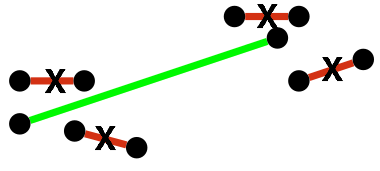
\includegraphics[scale=0.4]{gfx/ConstClust/Inform/Inform} 
	\caption[Informative constraint set.]{Informative constraint set \cite{davidson2007survey}}\label{fig:Informativity}.
\end{figure}


Informativity is estimated using the constraint set as a test set, so the ability of the algorithm to predict the constraints present in it is measured. Formalizing, given a set of constraints $CS$ and a constrained clustering algorithm $A$, we get the partition $P_A$ by applying the algorithm to the input dataset specifying an empty constraint set. We can compute the number of unsatisfied constraints in $P_A$ a in Equation \ref{eq:Informativity} \cite{davidson2007survey}.

\begin{equation}
I_A(R) = \frac{1}{|R|}\left[ \sum_{r \in R} unsat(r, P_A) \right] 
\label{eq:Informativity}
\end{equation}

\textbf{Coherence} measures the degree of agreement within the set of constraints itself with respect to a given metric ($D$). For instance, Figure \ref{fig:Coherence} shows two parallel and very close constraints of different type. It is in cases like this that the contradiction occurs, as the \acf{ML} constraints indicate that distance between instances involved in them is small, while \acf{CL}s indicate the opposite.

\begin{figure}[!h]
	\centering
	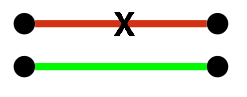
\includegraphics[scale=0.4]{gfx/ConstClust/Coherencia/Coher1}
	\caption[Non-coherent constraint set.]{Non-coherent constraint set. \cite{davidson2007survey}}\label{fig:Coherence}
\end{figure}

Then, the coherence measure is given by the degree of overlap that constraints produce by interpreting them as vectors in space and projecting them along one of the axes, as shown in Figure \ref{fig:CoherenceOverlap}.

\begin{figure}[!h]
	\centering
	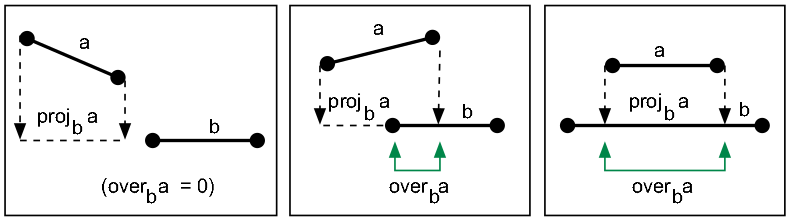
\includegraphics[scale=0.4]{gfx/ConstClust/Coherencia/Coher2}
	\caption[Coherence measure representation.]{Coherence measure representation. \cite{davidson2007survey}}\label{fig:CoherenceOverlap}
\end{figure}

\section{Summary}

Constrained clustering adds a new type of information to the original clustering problem, which is given in the form of specifications of belonging to the same or to different clusters on pairs of instances. Constraints, whether if they are the pairwise \acf{ML} and \acf{CL} constraints, or the distance-based $\delta$ and $\epsilon$ constraints, they are used to guide the clustering method we apply to a dataset in the search for a result partition that meets certain desired characteristics.

Clustering methods derived from this concept have proved to be very useful in many areas, as well as they present some problems that can be solved by deeply studying the constraints to be used to solve each individual problem.


































